\documentclass[sigplan,screen]{acmart}

\usepackage{graphicx}
\usepackage{amsmath}
\usepackage{algorithm}
\usepackage{algorithmic}
\usepackage{listings}
\usepackage{color}
\usepackage{soul}
\usepackage{listings}
\usepackage{hyperref}
\usepackage{subfigure}

\setcopyright{acmcopyright}
\copyrightyear{2022}
\acmYear{2022}
\acmDOI{XXXXXXX.XXXXXXX}

\acmConference[UM EECS 583 F'22]{University of Michigan EECS 583 Advanced Compilers Fall 2022}
{Dec 14, 2022, Ann Arbor, MI, USA}

% Title Page
\title{Isothermal Speculative Partial Redundancy Elimination}

% insert more authors like this
\author{Brent George}
\email{bdgeorge@umich.edu}
\affiliation{%
	\institution{University of Michigan}
	\streetaddress{2260 Hayward Street}
	\city{Ann Arbor}
	\state{Michigan}
	\country{United States}}

\author{Sahil Surapaneni}
\email{ssurapan@umich.edu}
\affiliation{%
	\institution{University of Michigan}
	\streetaddress{2260 Hayward Street}
	\city{Ann Arbor}
	\state{Michigan}
	\country{United States}}

\author{Priya Thanneermalai}
\email{tpriya@umich.edu}
\affiliation{%
	\institution{University of Michigan}
	\streetaddress{2260 Hayward Street}
	\city{Ann Arbor}
	\state{Michigan}
	\country{United States}}

\author{Gretchen Zheng}
\email{zhengji@umich.edu}
\affiliation{%
	\institution{University of Michigan}
	\streetaddress{2260 Hayward Street}
	\city{Ann Arbor}
	\state{Michigan}
	\country{United States}}


\begin{document}

	\begin{abstract}	
		Partial Redundancy Elimination(PRE) is a standard program optimization that removes redundant computations via Code Motion. Traditional PRE is very conservative and does not account for hot or cold paths in the code. This causes traditional PRE implementations to miss potentially lucrative optimization opportunities. In our final project, we intend to implement a novel and efficient optimization of PRE: Isothermal Speculative Partial Redundancy Elimination(ISPRE), as proposed by R. Nigel Horspool et al \cite{ispre_paper}. While the classical PRE analysis is performed without any knowledge of the relative frequencies of execution of the different paths, ISPRE takes advantage of the program profiling information and is executed as an approximate technique of the classic code motion method. Our results show speedup over several benchmarks, as well as optimizing test cases that are ignored by traditional PRE.
	\end{abstract}
	
	
	\maketitle
	
	\section{Introduction}
	\label{sec:introduction}

    Traditional Partial Redundancy Elimination is an optimization that allows for more aggressive use of redundancy elimination in the code.

    Redundancy elimination is the process of removing redundant computation that may be found across basic blocks in the code. For example, if 50 * 50 is computed twice, the compiler can change the IR to compute it just once and copy this result to the two desired destinations. This can provide incremental gains in overall run time with nearly zero code size expansion.

    Traditional PRE has two main limitations \cite{pre_paper}. The first is that front-end compilers can modify naming of variables in unique ways that may obscure potential redundant computations. The second is that the code shape, such as decisions about associativity and ordering of computational chains, can make certain redundancies non-obvious. Briggs and Cooper attempt to partially address these concerns in 1994 with global value numbering and global reassociation \cite{pre_paper}.

    Global value numbering has since become a common strategy to improve the scope of PRE. The gvn pass in the LLVM compiler (gvn) is a library pass that combines global value numbering with redundant load elimination. The gvn pass is included in the O2 (and higher) levels of optimization in clang and gcc.

    PRE is traditionally applied very conservatively. Traditional PRE does not use any profiling data, and will not optimize hot paths at the expense of cold paths - it will only optimize if there is no code size increase for any path. This can lead to missed optimization opportunities when considering control flows. Refer to \ref{fig:figure1} and \ref{fig:figure2} for an example of a case where PRE cannot optimize code, but ISPRE could. Since PRE has no knowledge of profiling data it cannot know whether hoisting up \(a*a\) will result in code speed up or slow down so it must ignore it.
    
    \begin{figure}[ht]
    \begin{minipage}[b]{0.45\linewidth}
    \centering
    \begin{small}
    \begin{verbatim}
    for(int i = 0; i< n; i++){
        if(i%200 == 0){
            a = i;
        }else{
            sum = a*a;
        }
    }
    \end{verbatim}
    \end{small}
    \caption{Code that PRE cannot optimize}
    \label{fig:figure1}
    \end{minipage}
    \hspace{0.5cm}
    \begin{minipage}[b]{0.45\linewidth}
    \centering
    \begin{small}
    \begin{verbatim}
  int t1 = a*a;
    for(int i = 0; i< n; i++){
        if(i%200 == 0){
            a = i;
            t1 = a*a;
        }else{
            sum = t1;
        }
    }
    \end{verbatim}
    \end{small}
    \caption{Optimized Code after ISPRE}
    \label{fig:figure2}
    \end{minipage}
    \end{figure}

    Speculative partial redundancy elimination (SPRE) is a technique that explicitly uses profiling information to find more aggressive optimization opportunities. It can be very effective, but very complex and difficult to implement, and as such many compilers stick to traditional PRE passes even if SPRE can provide large performance gains.

    SPRE is much more computationally expensive than PRE as well. Its analysis time can be very long compared to other code motion optimizations. Due to the complexity of SPRE's implementation, and the computational expense, Horspool et al. developed a novel approach called Isothermal Speculative Partial Redundancy Elimination (ISPRE) that delivers results similar to SPRE in practice, yet its analysis time is at least as good as current compiler techniques for code motion \cite{ispre_paper}. Our project is an implementation of ISPRE as described in their paper, as realized in a custom LLVM pass. 

    \section{Methods}
	\label{sec:methods}

    ISPRE uses dataflow analyses (similar to PRE) therefore bridging the gap between the faster speeds of PRE compared the SPRE and the better results of SPRE. In fact, as we will demonstrate in our results, in most cases ISPRE is faster than normal PRE. ISPRE uses profile information to divide a CFG $G$ into two subgraphs - a hot region $G_{hot}$ consisting of the nodes and the edges executed more frequently than a given threshold frequency $\theta$, and a cold region $G_{cold}$ consisting of the remaining nodes and edges. It is important to note that these hot and cold regions can be composed of multiple disconnected components of the CFG.
 
    \[G_{hot} = <N_H, E_H>\]  
    \[G_{cold} = <N_C, E_C>\]

    Where \(N_H , E,H\) are the hot nodes and edges and \(N_C , E,C\) are the cold nodes and edges respectively. We can then define the set of Ingress edges as

    \[{Ingress} = \{(u,v)\;|\;u \in N_C \wedge v \in N_H \}\]

    Essentially, the Ingress edges consist of all the edges in the program that flow from cold to hot regions of the CFG. ISPRE works by inserting expressions on edges in the Ingress set, which will then make some expressions in hot nodes become fully redundant. If those fully redundant expressions are then replaced by references to previously saved values of those same expressions, we have achieved code motion from $G_{hot}$ to $G_{cold}$. This may increase the code size, but will optimize the hot path and lead to runtime performance gains.

    This code motion is performed based on the results of two analyses: removability and necessity. Removability determines instances of computations in the hot region than can be deleted, and necessity determines edges in the Ingress set where these deleted computations must be inserted to maintain correctness of the code. Both of these analysis can be performed through dataflow analysis. 

    \subsubsection{Removability Analysis}

    Removability analysis can be done by computed XUse, Gen, and Kill sets for each basic block in a function (or loop, or whatever scope you determine. Our implementation is a LLVM FunctionPass, and so analyses functions independently). These sets inform a forward dataflow analyses that create a set of removable expressions. The following equations define each of these terms. 
    
    \begin{multline}
    \textrm{XUSES}(b) \overset{def}{=} \{\ e\ | \textrm{ expression } e \textrm{ occurs in } b \textrm{ and is not }\\ \textrm{preceded by any redefinitions of operands of } e\ \}
    \end{multline*}
    \begin{multline*}
    \textrm{GEN}(b) \overset{def}{=} \{\ e\ | \textrm{ expression } e \textrm{ occurs in } b \textrm{ and is not }\\ \textrm{followed by any redefinitions of operands of } e\ \}
    \end{multline*}    
    \begin{multline*}
    \textrm{KILL}(b) \overset{def}{=} \{\ e\ | \textrm{ block } b \textrm{ contains a statement which } \\ \textrm{maybe redefine an operand of } e\ \}
    \end{multline}
     
    \begin{multline}
    \forall b \in N:\\
        \textrm{AVOUT}(b) = (\textrm{AVIN}(b) - \textrm{KILL}(b)) \cup \textrm{GEN}(b)\\
        \tab\textrm{AVIN}(b) = \underset{p \in preds(b)}{\bigcap}
    \begin{cases}
      \text{Candidates} & \text{if $(p,b) \in $ Ingress}\\
      \text{AVOUT}($p$)& \text{otherwise}
    \end{cases}  
    \end{multline}
    \begin{multline}
    \forall b \in N_H:\\  
    \textrm{Removable}(b) = \textrm{AVIN}(b) \cap \textrm{XUSES}(b)
    \end{multline}

    \subsubsection{Necessity Analysis}
    
    The solutions for the \emph{Removable} sets assume that computations of all candidate expressions are available on the \emph{Ingress} edges. However, some candidate expressions are not necessary to insert on the ingress edges as they might be useless or redundant. 

    Necessity analysis is thus conducted to compute which expressions are required to be inserted on the ingress edges to maintain correctness. The set of expressions to be inserted on each ingress edge can be computed by backwards dataflow analyses, using the following equations.

    \begin{multline*}
    \forall b \in N_H:\\
    \textrm{NEEDIN}(b) = (\textrm{NEEDOUT}(b) - \textrm{GEN}(b)) \cup \textrm{Removable}(b)\\
    \textrm{NEEDOUT}(b) = \underset{s \in succs(b)}{\bigcup} \textrm{NEEDIN}(s)
    \end{multline*}
    \begin{multline*}
    \forall (u,v) \in \textrm{Ingress}:\\  
    \textrm{Insert}(u,v) = \textrm{NEEDIN}(v) - \textrm{AVOUT}(u)
    \end{multline*}

    \subsection{Multipass ISPRE}
    The methodology described above details a Single Pass ISPRE implementation. However, after the code motion resulting from the process above, we can apply subsequent passes of ISPRE with lower thresholds, \(\Theta\) in order to find other regions of code or other instructions where code motion could be beneficial. By lowering \(\Theta\) we select a larger \(G_{HOT}\), then ISPRE will again move code from the hot region to the cold region, thus improving program performance. The algorithm for how we implemented Multipass ISPRE is as follows 
    \begin{algorithm}[]
\caption{Multipass ISPRE}}\label{alg:cap}
   \begin{algorithmic}
   \STATE $\Theta \gets \text{0.9 * } \textit{maximum block count}$
   \STATE $passCount \gets 0$
   \REPEAT
   \STATE \textit{ISPRE}\textbf{ (CFG) }
   \STATE $\Theta \gets \Theta / 2$
   \STATE $passCount \gets passCount + 1$
   \UNTIL{$passCount = \text{number of desired iterations}$}
    \end{algorithmic}
    \end{algorithm}


    \section{Results}
	\label{sec:results}

    \subsection{Experimental Setup}
    Our goal was to test two seperate things: 1) how ISPRE performs with respect to GVN (LLVM's built in Partial Redundancy Elimination Pass) and 2) how Multipass ISPRE performs as we increase the number of iterations we run ISPRE. In order to test the first part, we created four custom C files as test cases, listed in the appendix (Section \ref{app:code}). We compiled each once with just the LLVM Global Value Numbering (GVN) and Dead Code Elimination passes, and once with just our custom ISPRE pass and dead code elimination pass (link to code listed in Section \ref{app:code}). To determine how ISPRE performs against GVN, we measured runtime, compile time, and IR bitcode size for both optimizations. The data displayed is the average of 10 runs for each test case. The results are listed in Table \ref{tab:resultssingle}. To test the second part, we created 3 slightly more complex C programs in which long dependency chains could potentially highlight the benefits of a multipass optimization (also listed in Section \ref{app:code}). On each of the test programs, we ran GVN, Singlepass ISPRE, and then Multipass ISPRE with 2, 3, and 4 iterations. We tested multiple number of iterations in order to asses the cost to reward ratio for increasing the number of passes in Multipass ISPRE. Similarly to the first test, we measured runtime, compile time, and bitcode size for all 5 passes. The results are listed in Tables \ref{tab:resultmultiruntime}, \ref{tab:resultmulticompiletime}, \ref{tab:resultmultisize}. Please note that in the results, the number in parentheses next to Multipass is the number of iterations ISPRE was run using the algorithm. 

    \subsection{Discussion}

    In the Singlepass ISPRE vs GVN test, we can see that ISPRE outperforms GVN across the tests as GVN cannot perform optimizations on those programs without the knowledge of branch weights. Across the 4 programs, ISPRE saw an average runtime decrease of \textbf{41.3\%} and a compile time decrease of \textbf{39.5\%} at the slight cost of a \textbf{0.497\%} increase in IR bitcode size. The slight increase in size is caused by the incurred overhead of adding fix up code during code motion between hot and cold regions. Regardless, the significant gains in runtime and compile time show the merit of incorporating profiling information in partial redundancy elimination optimization.

    The underlying code motion is demonstrated by Figures \ref{fig:no_ispre_cfg} and \ref{fig:ispre_cfg} in the Appendix. Code motion of an expensive multiply operation has been achieved from hot node $if.else$ into cold node $if.then$.

    In the Multi-pass ISPRE test, the results stay consistent with the findings of the original paper and the single pass test. Both single pass and multi-pass ISPRE outperform the GVN pass, though not as drastically as in the first test. Across the three tests, when comparing GVN to single pass ISPRE, we see a 21.1\% decrease in runtime and a 33.7\% decrease in compile time with a negligible decrease in size. When comparing single pass ISPRE to 2 iterations of multi-pass ISPRE, there is a 3.63\% decrease in runtime and a 14.2\% increase in compile time with a 1.19\% increase in size. From 2 iterations of multi-pass to 3 iterations, there is a 1.24\% decrease in runtime and a 16.4\% increase in compile time with a 1.51\% increase in size. The same trend of diminishing return can be observed between 3 and 4 iterations as well. Considering the added costs in compile time and size, heuristics could be helpful in navigating the tradeoff between runtime performance and compile time and size for multi-pass ISPRE. 
    
    \clearpage
    \begin{table}[!t]
	\begin{tabular}{|l|l|l|l|l|l|l|}
	\hline
	Test Case & GVN Runtime  & GVN Compile Time & GVN IR Size & ISPRE Runtime & ISPRE Compile Time & ISPRE IR Size \\ \hline \hline
	ISPRE\_1  & 0.354s & 7.5ms & 3504b & 0.288s & 4.9ms & 3524b \\ \hline
	ISPRE\_2  & 0.376s & 13.5ms & 3504b & 0.185s & 6.3ms & 3524b \\ \hline
	ISPRE\_3  & 0.061s & 8.5ms & 3932b & 0.022s & 6.8ms & 3984b \\ \hline
	ISPRE\_4  & 0.376s & 8.0 ms & 3524b & 0.189s & 4.7ms & 3540b \\ \hline
	\end{tabular}
	\caption{Test Results Against Custom Benchmarks}
	\label{tab:resultssingle}
	\end{table}

        \begin{table}[t!]
	\begin{tabular}{|l|l|l|l|l|l|}
	\hline
	Test Case & GVN  & Singlepass & Multipass(2) & Multipass(3) & Mutlipass(4)\\ \hline \hline
	MULTI\_1  & 1.257s & 1.201s & 1.172s & 1.162s & 1.159s \\ \hline
	MULTI\_2  & 1.395s & 1.384s & 1.342s & 1.314s & 1.308s \\ \hline
	MULTI\_3  & 1.485s & 0.678s & 0.662s & 0.661s & 0.627s \\ \hline
	\end{tabular}
	\caption{Execution Times of GVN, Singlepass ISPRE, and Multipass ISPRE}
	\label{tab:resultmultiruntime}
	\end{table}

       \begin{table}[t!]
	\begin{tabular}{|l|l|l|l|l|l|}
	\hline
	Test Case & GVN  & Singlepass & Multipass(2) & Multipass(3) & Mutlipass(4)\\ \hline \hline
	MULTI\_1  & 7.5ms & 5.6ms & 6.4ms & 7.5ms & 9.7ms \\ \hline
	MULTI\_2  & 7.9ms & 5.1ms & 6.0ms & 7.3ms & 10.2ms \\ \hline
	MULTI\_3  & 9.1ms & 6.2ms & 6.9ms & 8.3ms & 9.6ms \\ \hline
	\end{tabular}
	\caption{Compile Times of GVN, Singlepass ISPRE, and Multipass ISPRE}
	\label{tab:resultmulticompiletime}
	\end{table}

         \begin{table}[t!]
	\begin{tabular}{|l|l|l|l|l|l|}
	\hline
	Test Case & GVN  & Singlepass & Multipass(2) & Multipass(3) & Mutlipass(4)\\ \hline \hline
	MULTI\_1  & 3244b & 3248b & 3288b & 3336b & 3376b \\ \hline
	MULTI\_2  & 3360b & 3344b & 3392b & 3428b & 3468b \\ \hline
	MULTI\_3  & 3876b & 3864b & 3900b & 3940b & 3980b \\ \hline
	\end{tabular}
	\caption{IR Bitcode Size of GVN, Singlepass ISPRE, and Multipass ISPRE}
	\label{tab:resultmultisize}
	\end{table}
    
  \section{Future Work}
	\label{sec:futureWork}
 Though our pass is not as computationally intensive as Speculative PRE, there are still a few improvements that we could make to our ISPRE pass. As mentioned before, the multi-pass optimization could benefit from heuristics regarding when it should be applied, for how many iterations, and how \(\Theta\) should change between iterations.

 Building upon this idea, another improvement that we suggest is exploring the importance of the hot/cold threshold \(\Theta\). Further research can be done on tuning this hyper parameter to determine the optimal value across a broad spectrum of test cases as the split of hot and cold regions can have a drastic impact on the performance of ISPRE.

 Other future work includes analysis of register pressure and lifetime issues, and incorporating unsafe expressions into the framework.

\clearpage

 

 \section{Appendix}
	\label{sec:appendix}

 \subsection{Source Code}
 \label{app:code}

 Full source code for the LLVM pass, benchmarks, and tests can be found on GitHub (\url{https://github.com/bd-g/isothermal-speculative-pre/}).

\lstinputlisting[label = {alg:ispre_test1}, caption = {ISPRE\_1 Test Case Source Code}]
{ispre_test1.c}

\lstinputlisting[label = {alg:ispre_test2}, caption = {ISPRE\_2 Test Case Source Code}]
{ispre_test2.c}

\lstinputlisting[label = {alg:ispre_test3}, caption = {ISPRE\_3 Test Case Source Code}]
{ispre_test3.c}

\lstinputlisting[label = {alg:ispre_test4}, caption = {ISPRE\_4 Test Case Source Code}]
{ispre_test4.c}

\lstinputlisting[label = {alg:multi_test1}, caption = {MULTI\_1 Test Case Source Code}]
{multi_test1.c}

\lstinputlisting[label = {alg:multi_test2}, caption = {MULTI\_2 Test Case Source Code}]
{multi_test2.c}

\lstinputlisting[label = {alg:multi_test3}, caption = {MULTI\_3 Test Case Source Code}]
{multi_test3.c}

\subsection{Control Flow Graphs}

See Figures \ref{fig:no_ispre_cfg} and \ref{fig:ispre_cfg}.

\begin{figure*}[h]
\begin{center}
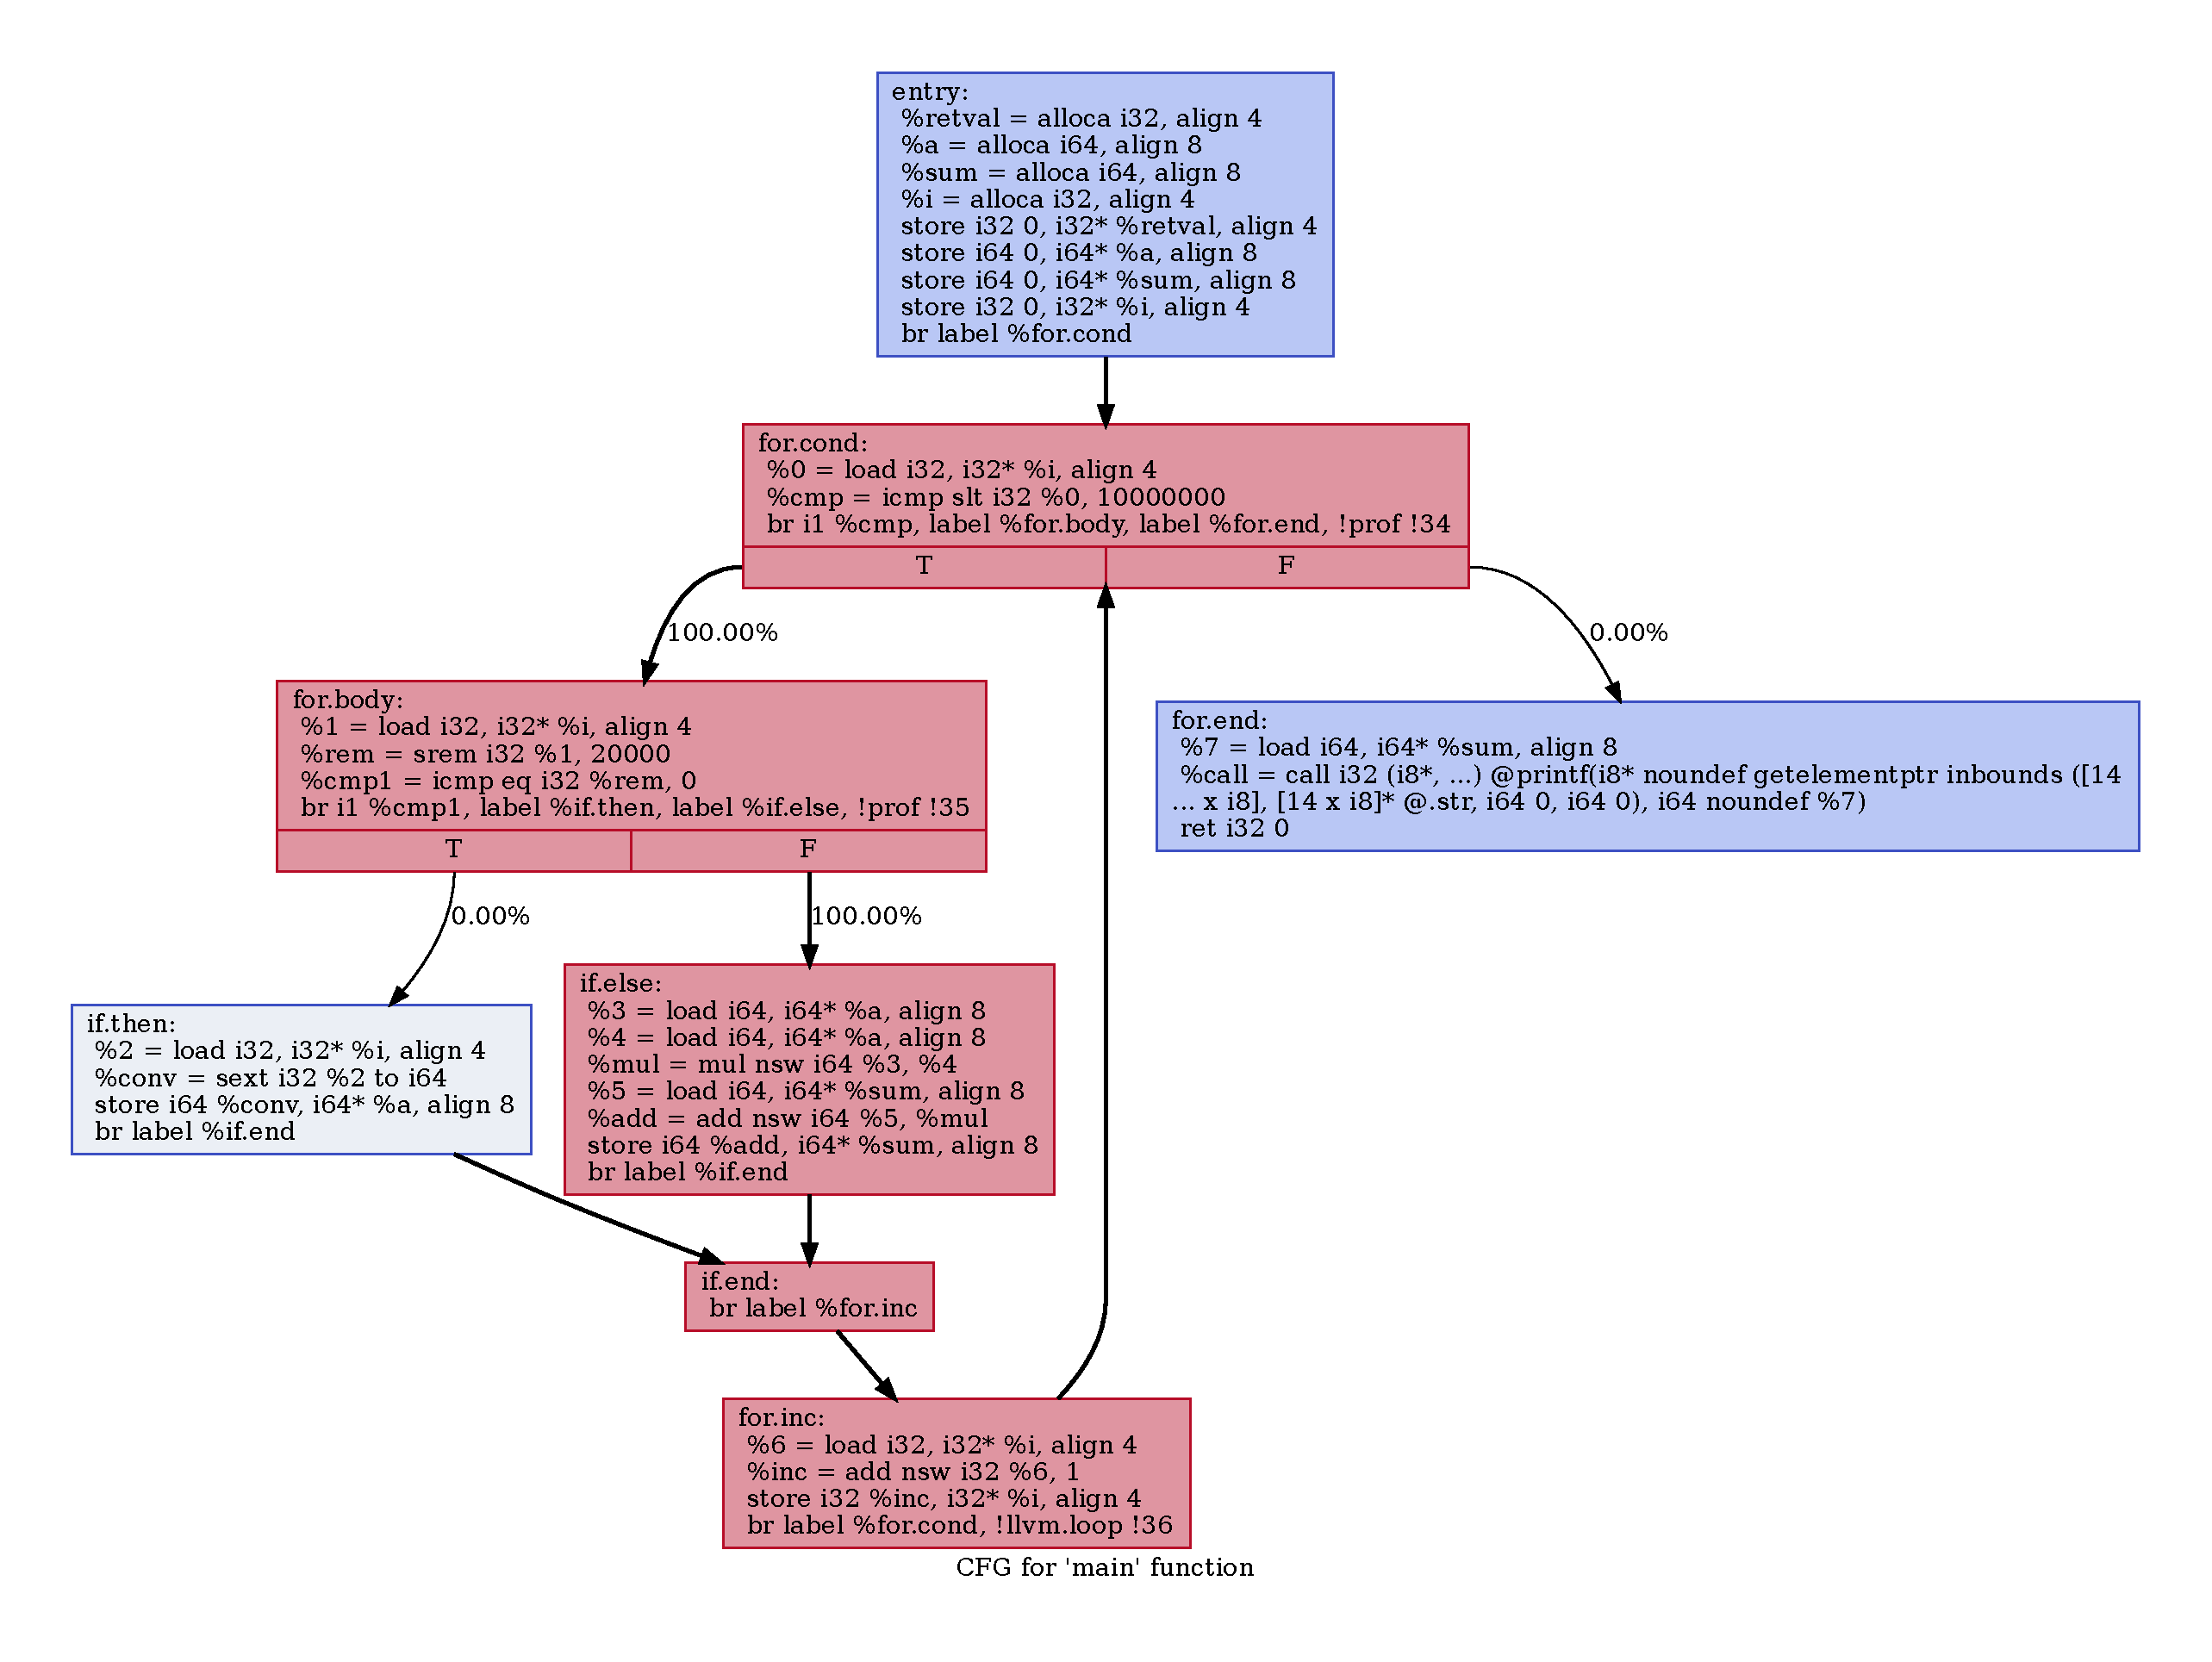
\includegraphics[width=0.95\linewidth]{ispre_test1.cfg.pdf}
\caption{CFG of Test Case 1 Before Custom ISPRE Pass}
\label{fig:no_ispre_cfg}
\end{center}
\end{figure*}


\begin{figure*}
\begin{center}
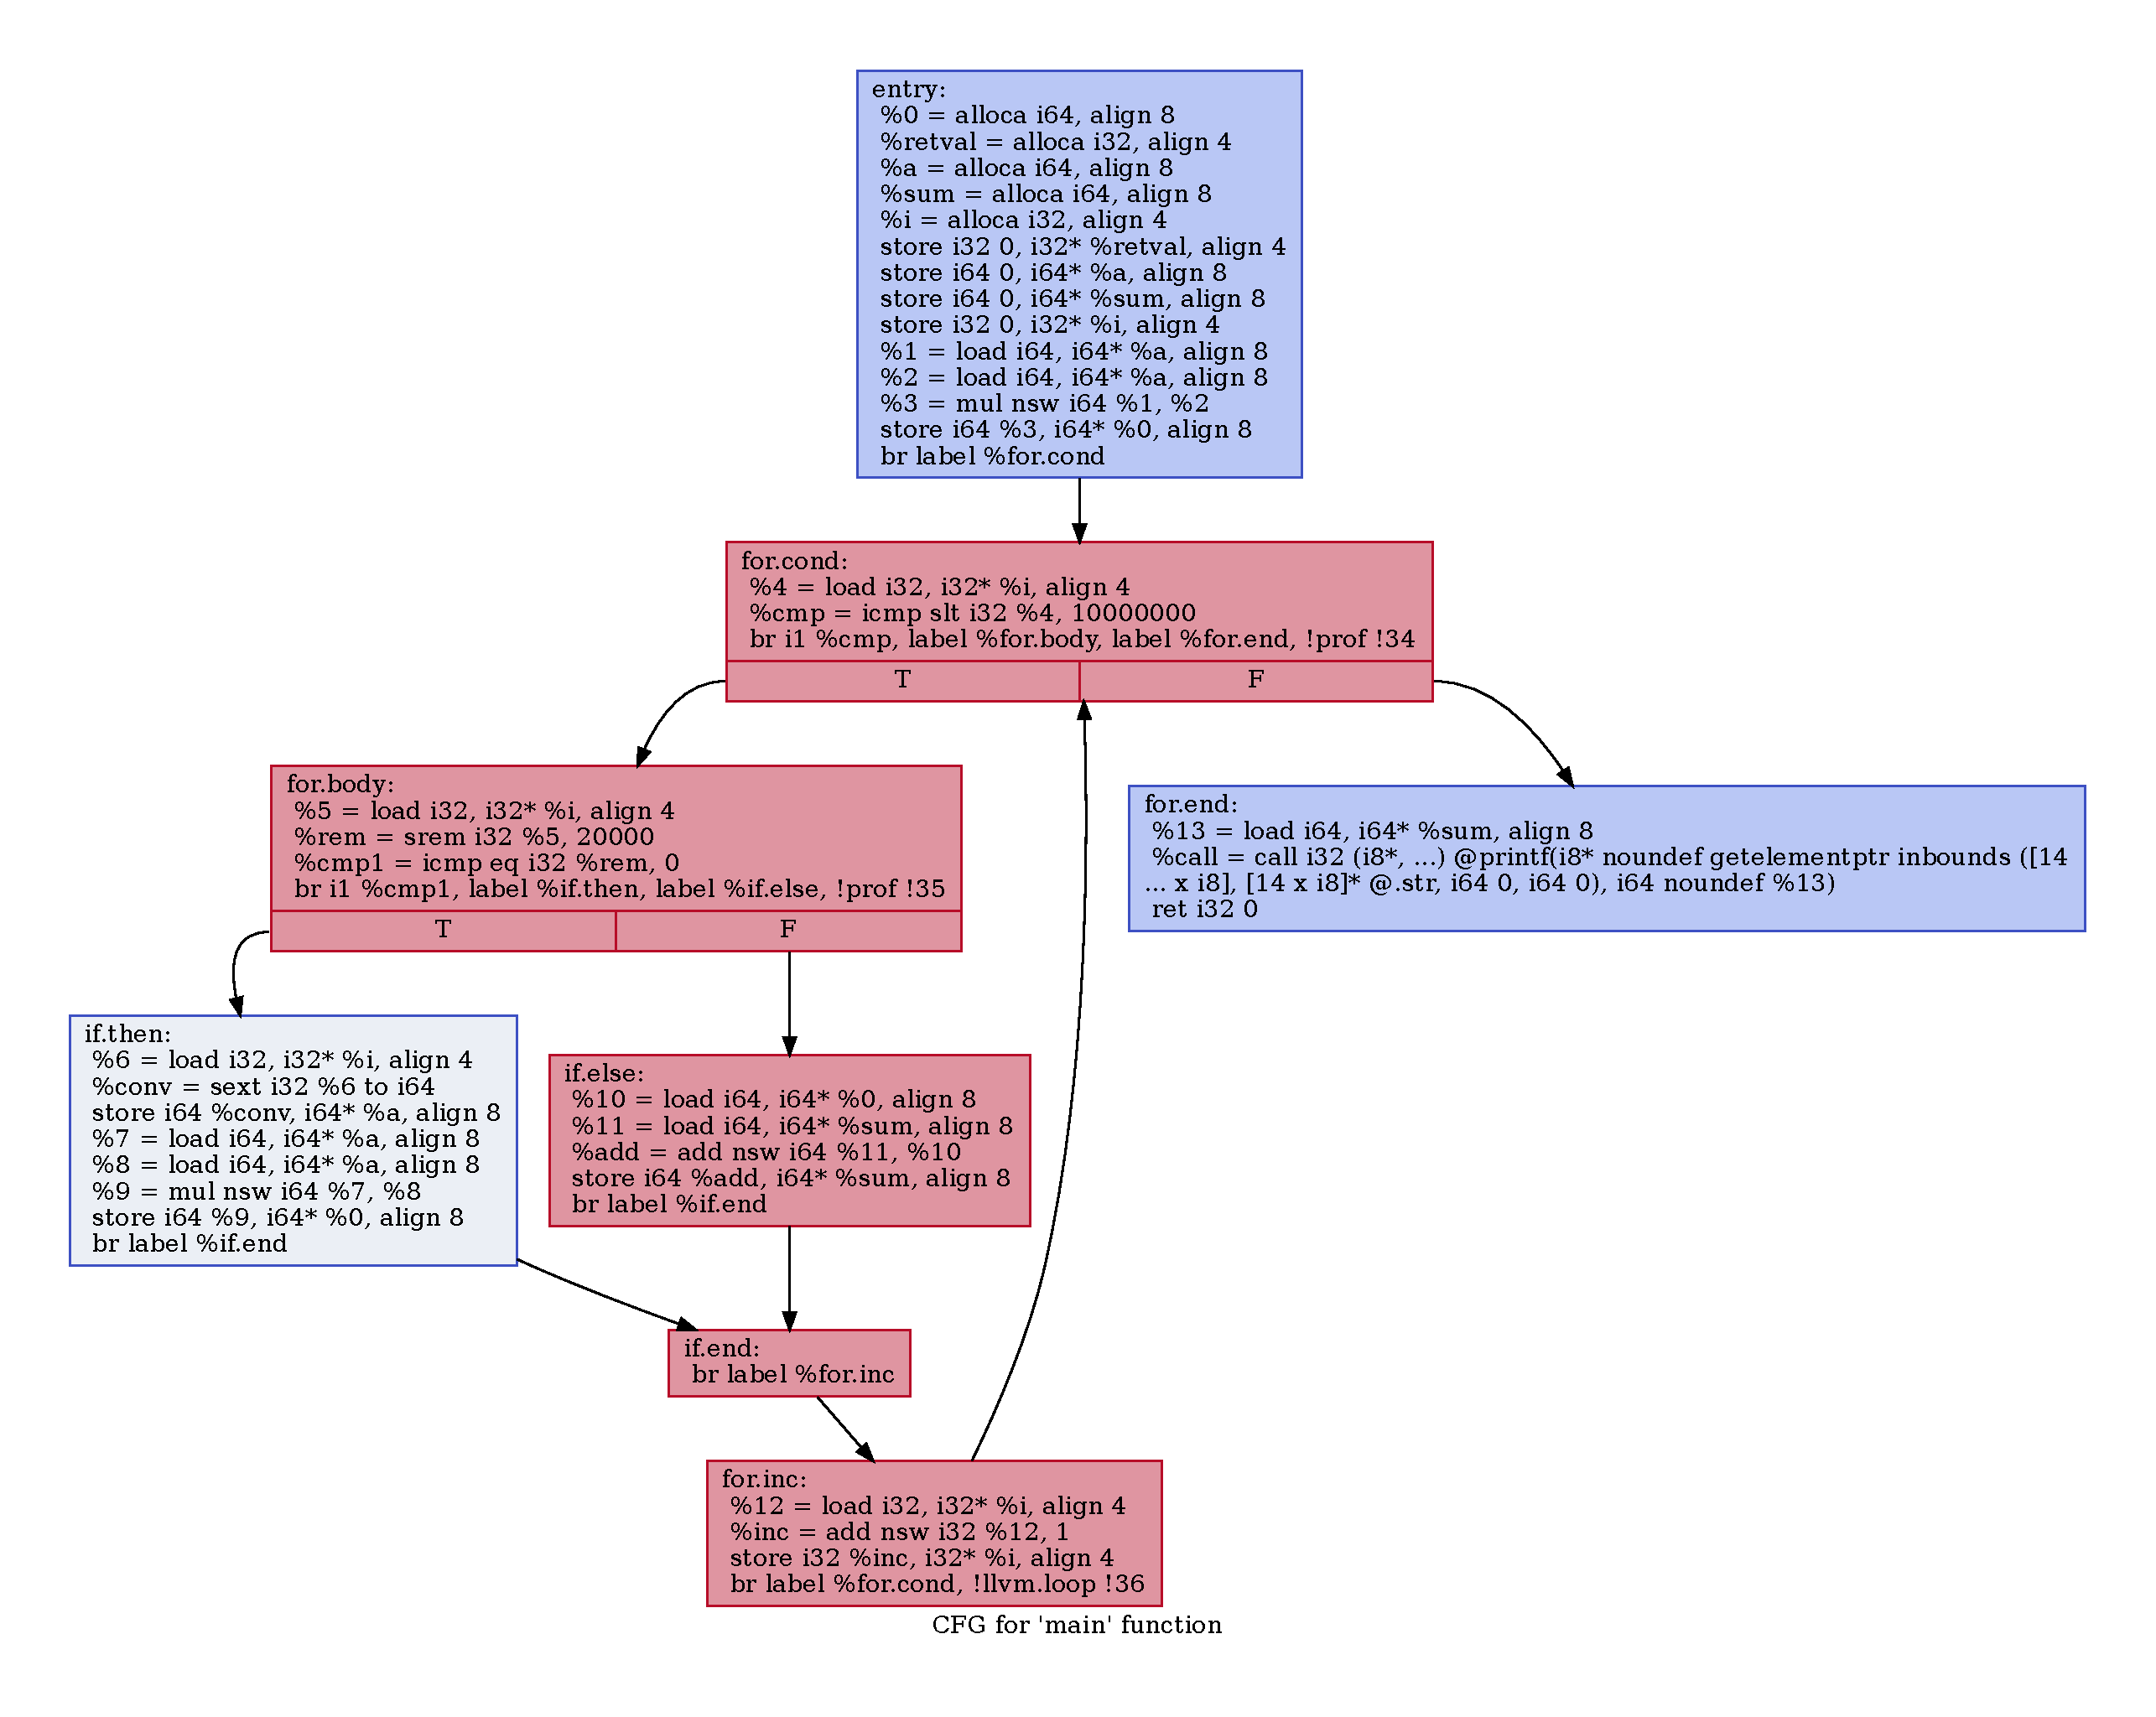
\includegraphics[width=0.95\linewidth]{ispre_test1.ispre.cfg.pdf}
\caption{CFG of Test Case 1 After Custom ISPRE Pass}
\label{fig:ispre_cfg}
\end{center}
\end{figure*}
 
	\bibliographystyle{plain}
	\bibliography{reference}

\end{document}          

